\documentclass[aspectratio=169,t]{beamer}
\usepackage[utf8]{inputenc}
\usepackage[T1]{fontenc}


\title{Mobile Anwendungen im Gesundheitswesen}
\date{WS 2019/2020}
\author[PWD]{Prof. Dr.-Ing. Piotr Wojciech Dabrowski}
\titlegraphic{Bilder/logo.png}
% https://pxhere.com/en/photo/1441931

\usepackage{HTWBeamerTemplate/beamerthemeHTW}
\subtitle{0: Allgemeines}
\addbibresource{Bilder/0/imagesources.bib}
\begin{document}

\setbeamertemplate{footline}[first]
\begin{frame}[noframenumbering]
\titlepage
\end{frame}

\setbeamertemplate{footline}[presentationbody] 

\begin{frame}{Vorstellung}
 \begin{itemize}
     \item<2-> Kurz zu mir
     \only<2-4>{
      \begin{itemize}
        \item<2-4> Kontakt: Piotr.Dabrowski@htw-berlin.de - gerne nutzen!
        \item<2-4> Repository: https://github.com/dabrowskiw/
        \item<3-4> Geboren 1981 in Warschau
        \item<3-4> Studium der Biotechnologie \& Informatik an der TU Berlin
        \item<3-4> Promotion über Auswertung von Hochdurchsatzdaten für Virus-Diagnostik
        \item<3-4> Aufbau der bioinformatischen Analytik für das NGS-Labor des RKI
        \item<3-4> Aufbau der Bioinformatics Core Facility am RKI
        \item<4> Hang zu unkonventionellen Vorlesungsmethoden - Feedback erwünscht!
      \end{itemize}
     }
     \note<4->{Erstes Mal Vorlesung, Background nicht in mobilen Applikationen\\
     Bitte um Geduld, Hinweise
     }
     \item<5-> Der Todesstern \& (ausgewählte) andere Hilfsmittel
     \item<9-> Sie \& Ihre Vorstellungen, Motivation und Vorkenntnisse
     \only<10->{
       \begin{itemize}
           \item Tafelbild - coming to a git repo near you starting tomorrow!
       \end{itemize}
     }
 \end{itemize}
 \only<5-8>{
  \begin{textblock}{15}(2,7)
   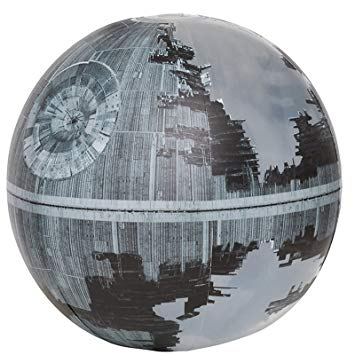
\includegraphics[width=3cm]{Bilder/0/Todesstern.jpg}
  \end{textblock}
 }
 \only<6-8>{
  \begin{textblock}{15}(5.5,8.25)
   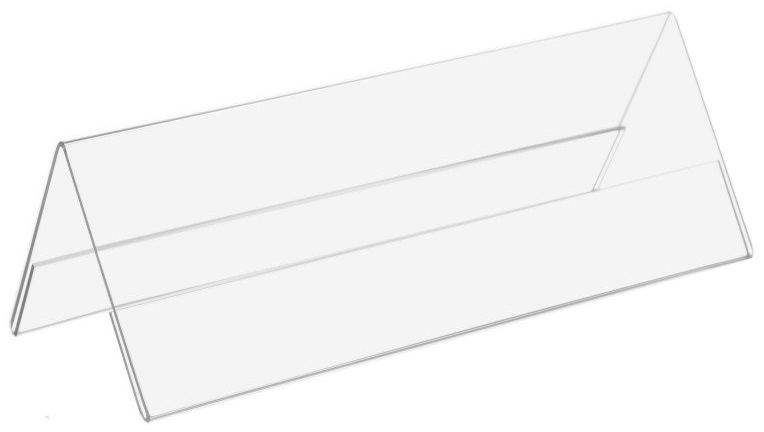
\includegraphics[width=3cm]{Bilder/0/Tischnamensschild.png}
  \end{textblock}
 }
 \only<7-8>{
  \begin{textblock}{15}(9,7.5)
   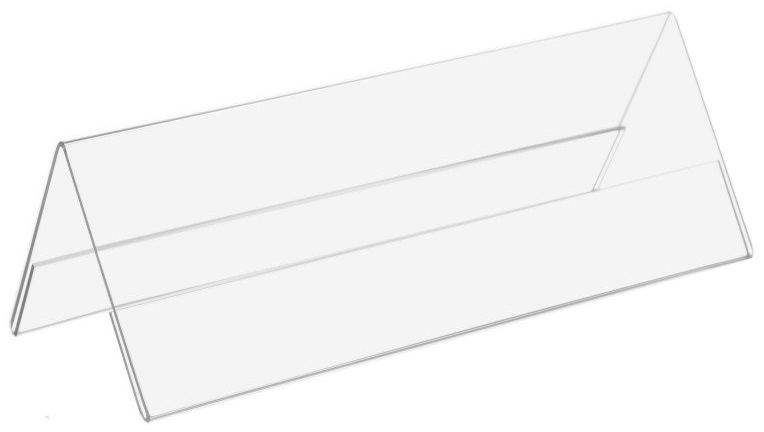
\includegraphics[angle=77,origin=c,height=2cm]{Bilder/0/Tischnamensschild.png}
  \end{textblock}
 }
 \only<8>{
  \begin{textblock}{15}(11.5,8)
   
\includegraphics[width=3cm]{Bilder/0/Whiteboard.png}
  \end{textblock}
 }
\end{frame}

\begin{frame}{Fragen der Vorlesung}
\note{
\begin{itemize}
    \item Entwicklung: Besonders wichtig bei Gesundheitswesen: Stabilität, einfache Anwendbarkeit (patient compliance)
    \item Was sind personenbezogene Daten, wann darf man sie verarbeiten - und wann sollte man sie verarbeiten etc.
\end{itemize}
}
\begin{itemize}
    \item Warum sind mobile Applikationen im Gesundheitswesen sinnvoll? Wo werden sie bereits eingesetzt?
    \item<2-> Worauf muss man bei der Entwicklung mobiler Applikationen für das Gesundheitswesen achten?
    \item<3-> Was sind Herausforderungen im Zusammenhang mit der Verarbeitung potentiell sensitiver Daten?
\end{itemize} 
\end{frame}

\begin{frame}{Inhalt der Übung}
\note{
    Produktpräsentation:
    \begin{itemize}
        \item Ideen, Herausforderungen, Umgehen mit Herausforderungen so darstellen, dass sie für die Anderen nachvollziehbar und nützlich sind!
        \item Vorstellung des PoC: Verkaufsevent, warum sind wir besser als alle anderen!
    \end{itemize}
}
Entwicklung einer mobilen medizinischen Applikation.
    \begin{itemize}
        \item<2-> Zusammenfinden in möglichst balancierten Teams (5 Personen)
        \item<3-> Entwickeln einer Produktidee
        \item<4-> Erstellung eines Mockups
        \item<5-> Implementation eines Proof of Concept
        \item<6-> Erstellung einer Produktpräsentation (15 Minuten/Gruppe)
    \end{itemize}
\end{frame}

\begin{frame}{Benotung}
 \note<2>{Muss nicht ``fertig werden'', Idee und Herangehensweise ausschlaggebend.}
 \begin{itemize}
     \item<1-> Klausur: $40\%$
     \item<2-> Code- und Repo-Qualität: $40\%$
     \only<3>{
        \begin{itemize}
            \item Dokumentation des Codes (Vorhandensein, Übereinstimmung Dokumentation/Code): $10\%$
            \item Konsistenter Code-Stil: $10\%$
            \item Vorhandensein dokumentierter Tests: $10\%$
            \item Kleinteilige Commits: $10\%$
        \end{itemize}
    }
     \item<4-> Ergebnisvorstellung: $20\%$
     \item<5-> Verbesserungsvorschläge/Fehlerkorrekturen
     \begin{itemize}
         \item $2.5\%$ pro Stück
	 \item Maximal 2 pro Semester
	 \item Wenn als pull request: Doppelte Punktzahl
     \end{itemize}
 \end{itemize}
\end{frame}

\begin{frame}{Sourcecode-Verwaltung}
Aus EGI
\end{frame}

\begin{frame}{Gesundheitswesen}
Aus EGI + Mobile Applikationen dazu
\end{frame}

\begin{frame}{Flutter}
\note{
Mini-Whiteboard: Was ist Wichtig bei der Entscheidung für eine Sprache für ein Projekt?
\begin{itemize}
    \item Entwickler: Einer? Mehrere? Community oder Spaltungen?
    \item Anzahl an reifen Projekten in Sprache
    \item Bekannte Schwachstellen und Reaktionen (exploitdb etcexploitdb etc)
\end{itemize}
}
 \begin{itemize}
     \item Wichtig in Programmierung: Weniger konkrete Sprache, mehr breites Wissen
     \note{Beispiele:\\Java super für portable, performante Applikationen, aber mies für Prototyping\\Python super für Prototyping, aber schlecht für Stabilität\\PHP Totalausfall bei Wartbarkeit+Sicherheit, aber toll für schnelle kleine Webapp\\Wünsche JavaScript schnellen und schmerzhaften Tod, setze es trotzdem für interaktive Visualisierungen ein\\etc... \\Fazit: Keine silver bullet, man muss viele Stärken und Schwächen kennen, und z.T. Programmierkonzepte zwischen Sprachen übertragbar. Flexibilität ist wichtig!}
     \item<2-> Flutter: Framework für die Entwicklung mobiler Applikationen
     \item<3-> Dart: Für flutter verwendete Sprache
     \item<4-> Von Google entwickelt und eingesetzt
     \item<4-> 
 \end{itemize}
\end{frame}

\begin{frame}{Live-Minimalbeispiel}
\end{frame}


\begin{frame}{Bildquellen}
\printbibliography
\end{frame}

\end{document}
